\documentclass[
	ruledheaders=section,%Ebene bis zu der die Überschriften mit Linien abgetrennt werden, vgl. DEMO-TUDaPub
	class=report,% Basisdokumentenklasse. Wählt die Korrespondierende KOMA-Script Klasse
	thesis={type=bachelor},% Dokumententyp Thesis, für Dissertationen siehe die Demo-Datei DEMO-TUDaPhd
	accentcolor=9c,% Auswahl der Akzentfarbe
	custommargins=true,% Ränder werden mithilfe von typearea automatisch berechnet
	marginpar=false,% Kopfzeile und Fußzeile erstrecken sich nicht über die Randnotizspalte
	%BCOR=5mm,%Bindekorrektur, falls notwendig
	parskip=half-,%Absatzkennzeichnung durch Abstand vgl. KOMA-Sript
	fontsize=11pt,%Basisschriftgröße laut Corporate Design ist mit 9pt häufig zu klein
%	logofile=example-image, %Falls die Logo Dateien nicht vorliegen
]{tudapub}


% Der folgende Block ist nur bei pdfTeX auf Versionen vor April 2018 notwendig
\usepackage{iftex}
\ifPDFTeX
\usepackage[utf8]{inputenc}%kompatibilität mit TeX Versionen vor April 2018
\fi

%%%%%%%%%%%%%%%%%%%
%Sprachanpassung & Verbesserte Trennregeln
%%%%%%%%%%%%%%%%%%%
\usepackage[english,ngerman, main=english]{babel}
\usepackage[autostyle]{csquotes}% Anführungszeichen vereinfacht
\usepackage{microtype}


%%%%%%%%%%%%%%%%%%%
%Literaturverzeichnis
%%%%%%%%%%%%%%%%%%%
\usepackage{biblatex}   % Literaturverzeichnis
\bibliography{thesis}
%\addbibresource{thesis.bib}


%%%%%%%%%%%%%%%%%%%
%Tabellen
%%%%%%%%%%%%%%%%%%%
%\usepackage{array}     % Basispaket für Tabellenkonfiguration, wird von den folgenden automatisch geladen
\usepackage{tabularx}   % Tabellen, die sich automatisch der Breite anpassen
%\usepackage{longtable} % Mehrseitige Tabellen
%\usepackage{xltabular} % Mehrseitige Tabellen mit anpassarer Breite
\usepackage{booktabs}   % Verbesserte Möglichkeiten für Tabellenlayout über horizontale Linien
\usepackage{makecell}
\usepackage{multirow}
\renewcommand\theadfont{\bfseries}

%%%%%%%%%%%%%%%%%%%
%Paketvorschläge Mathematik
%%%%%%%%%%%%%%%%%%%
%\usepackage{mathtools} % erweiterte Fassung von amsmath
%\usepackage{amssymb}   % erweiterter Zeichensatz
%\usepackage{siunitx}   % Einheiten


\usepackage{hyperref}
\usepackage{tikz}
\usepackage{listings}
\usepackage{subcaption}
\usepackage{amsmath}
\usepackage[justification=centering,labelfont=bf]{caption}
\usepackage{adjustbox}


%Formatierungen für Beispiele in diesem Dokument. Im Allgemeinen nicht notwendig!
\let\file\texttt
\let\code\texttt

\usepackage{pifont}% Zapf-Dingbats Symbole
\newcommand*{\FeatureTrue}{\ding{52}}
\newcommand*{\FeatureFalse}{\ding{56}}

\lstdefinelanguage{JavaScript}{
  morekeywords=[1]{break, continue, delete, else, for, function, if, in,
    new, return, this, typeof, var, void, while, with, await, async, case,
    catch, class, const, default, do, enum, export, extends, finally, from,
    implements, import, instanceof, let, static, super, switch, throw, try},
  % Literals, primitive types, and reference types.
  morekeywords=[2]{false, null, true, boolean, number, undefined,
    Array, Boolean, Date, Math, Number, String, Object},
  % Built-ins.
  morekeywords=[3]{eval, parseInt, parseFloat, escape, unescape},
  sensitive,
  morecomment=[s]{/*}{*/},
  morecomment=[l]//,
  morecomment=[s]{/**}{*/}, % JavaDoc style comments
  morestring=[b]',
  morestring=[b]",
  morestring=[b]`
}[keywords, comments, strings]

\lstset{
  language=JavaScript,
  basicstyle=\ttfamily,
  numbers=left
}

% these words should not by hyphenated
\hyphenation{postMessage}
\hyphenation{setTimeout}
\hyphenation{setInterval}



\begin{document}

\Metadata{
	title=Analysis of Methods for Background Execution in Modern Web Applications,
	author=Yannick Reifschneider
}

\title{Analysis of Methods for Background Execution in Modern Web Applications}
\subtitle{Analyse von Verfahren für Hintergrundausführung in modernen Webanwendungen}
\author[Y. Reifschneider]{Yannick Reifschneider}%optionales Argument ist die Signatur, 
\reviewer{Dipl.-Inf. Nikolay Matyunin \and Prof. Dipl.-Ing. Dr. Stefan Katzenbeisser}%Gutachter

%Diese Felder erden untereinander auf der Titelseite platziert. 
%\department ist eine notwendige Angabe, siehe auch dem Abschnitt `Abweichung von den Vorgaben für die Titelseite'
\department{inf} % Das Kürzel wird automatisch ersetzt und als Studienfach gewählt, siehe Liste der Kürzel im Dokument.
\institute{Security Engineering Group}
%\group{Security Engineering Group}
%\addTitleBoxLogo{SecEng_white}

\submissiondate{\today}
\examdate{\today}

%\tuprints{urn=1234,printid=12345}
%\dedication{I dedicate this thesis to my deceased sister Kimberly whose support and encouragement enriched my life and inspired me to pursue and complete my studies.}

\maketitle

\begin{abstract}
  The world wide web today is not only used for serving static pages of information but it is also used as a platform for sophisticated web applications. These web applications may be opened for long durations during everyday computing activities. Other reasearch shows, that there are many attacks against the web browser executed from malicous web sites. Some of these attacks assume a long uninterrupted timespan for execution, for example cryptocurrency miners or exploits targeting hardware-based vulnerabilities. Therefore these attacks greatly benefit from being executed from web applications, which are opened for a long time on the victims computer. However, most web browsers limit the time a web site can execute code, when the web site is not in focus for energy conserving reasons.

  In this thesis, we analyse modern browsers regarding their behaviour of JavaScript code exection in background tabs. We show that the energy conserving limits of background code execution of most browsers can easily be circumvented. We discuss and explain how the circumvention methods work and how browsers behaviour differ. For this research, we developed a framework for comparing and analysing different methods for background execution. This framework allows expansion for newly discovered methods as well as review of existing methods for new browser versions.

  With the findings from our research, we performed a dynamic analysis of popular web sites to measure their code execution in the background and determine if they use limit-circumventing techniques for achieving longer background execution. The result of this analysis shows that all web sites circumventing the browser limits use one or more methods we explained.

  To conclude, we discuss potential changes to browsers to prevent background code execution for web sites without explicit user consent.
\end{abstract}

\tableofcontents

\newpage

\chapter{Introduction}

Web technology received rapid advances in the last years. Many websites not only deliver static information in form of text and images, but instead modern web sites implement complex logic by executing JavaScript code on the client. This allows web sites to build highly dynamic applications which compete with traditional software products. For many of the standard business applications like an e-mail client, a word processor or even a bitmap graphic manipulation software there exist alterantives \cite{gmail}, \cite{office365-online}, \cite{photopea}, which are developed using web technologies and can be accessed via a modern web browser.

Some reasons for the rise of popularity of web applications are that the web platform is providing more powerful APIs every year and the performance of browsers is drastically increasing so that CPU intensive tasks are feasable to be implemented as web application. Developing a web application instead of traditional software has also many benefits for the developers and publishers of said software. Web applications do not need installation. They just require a modern web browser, which comes preinstalled with any common operating system or mobile device. Users always use the latest version, because it is not installed to the users hard drive, thus reducing support and maintanance cost. Visiting a web site to try out a piece of software is a much smaller hurdle to overcome then downloading, installing and running a piece of traditional software. These are some reasons which make the web a popular platform for development of new applications.

The web browser is a fundamental application on most personal computing devices and web browser usage is ubiquitous in everyday computing activities, because many modern applications are implemented as web apps. Also, users often use their browser with many tabs open at once \cite{weinreich2008not}. As such, browser vendors are encouraged to conserve as much energy as possible to enable users on battery powered devices, such as mobile phones or notebooks which are not tethered to a power outlet, a longer usage time. For maximum energy efficiency, all tabs in the background should eventually be halted completely, and only woken up when the page is moved to the foreground again. Suspending all background tabs is the stated goal of browser vendors \cite{chrome-background-tabs-roadmap}, but this change in behaviours is not yet implemented due to missing alternative APIs enabling the major use cases, which require background execution. Web apps, which need regular CPU time are sites, which notify the user about new content such as a news site or a social network, a web application which plays audio or video, or a web video conference application. For the time being, browsers only \textit{limit how often} web sites can schedule new work when a web site is not in focus to not break existing sites which are performing background tasks.

\textbf{TODO: restructure following paragraphs}

  Other research shows that


  In this thesis we find out, if the throttling mechanisms employed by browser vendors can be circumvented, so that web sites which are not visible to the browser can gain code execution for arbitrary time. We compare the different throttling mechanisms between desktop and mobile browsers and we trace popular websites to see if the found cirumvention methods are actively used in the wild.


  At the same time, the revenue model for many websites is advertising. Websites include third party JavaScript from ad networks, which display ads and track impressions. The included code can be controlled by the advertiser. For a malicous entity, it is therefore possible to include JavaScript on reputable websites just by paying for the ad impression. This method of distribution for malicous script is known as malvertising\cite{wiki:malvertising}.
 

  Nevertheless there are numerous activities, which malicous entities could perform with access to a web site with high amount of daily visits.

  \begin{itemize}
  \item The attacker could inject a browser crypto-currency miner to convert electricity of the website visitors into crypto currency. The existance of crypto currencies such as Monero, which uses proof of work algorithm, which is inefficient to calculate on custom hardware, makes the browser a viable target for such mining. Existing implementations of Monero miners implemented in web assemlby are available for this attack.
  \item The browser could be used as a compute node in a botnet, which can be used for DDoS attacks or for cracking hashed passwords. Grossman et al.\cite{grossmann2013million} show that these attacks can be used with standard web technologies and not exploiting any weaknesses.
  \item The computer of the visitor itself could be compromised by using exploits of the browser or the underlying system itself. Attacks which exploit hardware weaknesses such as Spectre\cite{Kocher2018spectre}, which could allow an attacker to read memory space of other browser tabs, could expose sensitive informations such as passwords or banking information of the uses. Rowhammer\cite{rowhammer} attacks could even persistently infect the users system. These exploits usually need quite some time to be successful and could benefit from constant background execution in a background browser tab.
  \end{itemize}

  \section{Goals}

  The goals of this thesis are threefold: First, we want to analyse how browsers throttle tasks in background tabs. Second, we try to find methods to circumenvent the throttling mechanisms put in place. And third, we analyse popular web sites to confirm whether these methods are used to actively or inadvertently circumvent the browser throttling. However, we are not investigating what these web sites do in the background, merely if and how long background tasks are executed. With this research, we contribute the answer to the question whether the current energy-saving mechanisms implemented by browsers are suitable to protect users from malicious background activites on rogue web sites.

  \section{Organization of this thesis}

  This thesis is organized into the following chapters:

  \begin{description}
  \item[Chapter 2] describes the basic principles of web scripting and how the JavaScript language handles tasks and concurrency.
    
  \item[Chapter 3] gives an overview of other research related to our field of study. We compare our research to prior work and highlight possible attacks targeting web browsers which assume some form of continous execution time.
    
  \item[Chapter 4] describes methods for performing tasks in background tabs. We analyse how each browser behaves in regards to their throttling mechanisms to each method and how the different browser implementations differ.
    
  \item[Chapter 5] is about dynamic analysis of popular web sites. We explain how the automated tracing of popular web sites was conducted and we describe the results of this analysis.
    
  \item[Chapter 6] discusses the result of our research and proposes changes to the behaviours of browsers to protect users from unwanted activities of background tabs.
  \end{description} 

  
  \newpage
  \chapter{Background}
  
  The development of modern web applications is done with JavaScript code, which gets embedded in the resources of the web site and is executed by the browser. The JavaScript language was originally designed as an extension to HTML (Hypertext Markup Language) and CSS (Cascading Style Sheets) which form the foundation of the world wide web. The goal was to enable simple user interaction with web pages like validation of user-entered form input. Although it is nowadays used for much more sophisticated web applications, the basic principle of the web did not change since: When a user visits a web site, the browser downloads all resources belonging to this web site, like HTML, images and also JavaScript code. These scripts are run to build up the complete website. When a user visit a web page and did not disable JavaScript execution, they implicitly allow this web site to execute code on their machine.

  Most desktop browsers also provide an alternative to run client applications on users machine via plugins such as Java Applets, Flash or Silverlight. However, these plugins are usually not supported by mobile browsers and the usage steadily declined since smartphones and mobile browsers became widely adopted. Today, JavaScript is the dominating technology for browser based applications \cite{browser-plugin-usage}.

  JavaScript is a scripting language. As such, it is not compiled to native machine code but it requires an interpreter which parses and executes the JavaScript code at runtime. All major browsers include an JavaScript interpreter to correctly display modern web sites. The HTML5 specification describes how JavaScript engines have to interoperate with the browser and which APIs the browser must expose to JavaScript code which is embedded in web sites \cite{html5-specification}.

  In the following sections, we describe how browsers run JavaScript code and how concurrency and long running tasks are handled in JavaScript.

  \section{The JavaScript execution context}

  Each browser tab creates a browsing context which allows interfacing with the opened web site. JavaScript code embedded in the web site can either be executed in this browsing context or another context created by this web site, e.g. a web worker. In this thesis we define \textbf{execution context} to refer to both a browsing context and other contexts in which JavaScript code is executed in.

  A JavaScript execution context is organized into a task queue, an event loop, a stack and a heap \cite{mdn-event-loop}.

  \begin{description}
  \item[Task queue] The task queue defines a list of tasks, which should be executed by the JavaScript runtime. A task consist of a callback function and optional arguments to this callback function.
  \item[Event loop] The JavaScript runtime implements an event loop, which processes the task queue. During the event loop, the runtime waits for tasks to be added to the task queue. When the task queue is not empty, the event loop removes the first task from the queue and executes its corresponding callback function with the provided arguments. This is repeated until the task queue is empty.
  \item[Stack] The stack is comparable to a call stack in other programming languages like Java or C. When a callback function from the task queue is executed, it creates a frame on the stack. Each function call inside the callback function also creates a stack frame. When a function returns, its frame is removed from the stack. A task from the task queue is finished, when the stack is empty.
  \item[Heap] The heap is a memory region for long living objects, which are not destroyed after the execution of a single task.
  \end{description}

  When a JavaScript task is running, it is guaranteed to not be interrupted until it is completed. This also insures, that every variable cannot be changed from outside during the execution of a task. This is in contrast to many other programming languages like Java or C, where another thread can mutate variables at any time. To guarantee this behaviour, the JavaScript runtime in the web browser has wait for task to finish before it can continue rendering the web page, because the JavaScript task has access to the browser internal state and Document Object Model (DOM).  The DOM describes the representation of a web page and provides an API for manipulation of the element tree and registration of event handlers.. Due to JavaScript code having access to these internal structures, tasks should be as small as possible to ensure responsiveness of the browser \cite{chrome-rail-model}. If a JavaScript task takes a long time to complete (i.e. it is executing an infinite loop) most browser show a warning to the user that a script is slowing down the website. The user then has the option to kill the task or wait for the task to finish.

  Tasks can be added to the task queue by registering event listeners for events, for example a onclick handler of a button. When this event occurs, the runtime then adds a new tasks to the task queue. Tasks can also be added by JavaScript code itself, for example by using a timer.

  
  \section{The JavaScript concurrency model}
  
  The JavaScript language does not support multi threading. Each browser tab has it's own JavaScript execution context. This execution context is tied to the rendering of the page, as explained in the section before. As long running JavaScripts tasks block the rendering of the web page, calls to potentially long running functions or other side effects are almost never blocking, but instead register a callback function to be called, when the result of function returns. The runtime then performs the side effect and creates a new task in the task queue with the registered callback function and the result of the side effect as a parameter for the callback. With this workaround it is possible to perform multiple long running tasks at the same time, by splitting the work into smaller tasks, which are suspended when they are waiting for other input and are resumed when the result becomes available.
  
  
  \section{Web workers}

  Web workers were an addition to the HTML5 specification, to overcome some of the limitations, which were described before. Web workers create a new execution context, which is \textit{not tied} to the browser rendering. They were introduced to perform long running uninterruptable calculations, which would block the rendering process for too long, if they would be executed in the main browser context. They don not share variables or resources with the main JavaScript context. The worker context therefore does not have access to the DOM of the web page, because that would introduce shared memory between the worker and main context, which would invalidate the runtime guarantees of the JavaScript specification. Other resources, such as network requests, which are independent from the main context are available to the worker context. The web worker and main thread context can communicate by passing messages to each other which are handled by their respective event loops. This allows the result of a calculation which happened in the worker context to be passed to the main context and then be made visible to the user by showing the result in the DOM.

  \section{Dynamic analysis of JavaScript code}
  \textbf{TODO: dynamic analysis}

  
  \newpage
  \chapter{Related work}

  \textbf{TODO: restructure to formal text instead of bullet points}

  \begin{itemize}

  \item Papadopoulos et al.\autocite{papadopoulos2018truth} analyses the if Cryptocurrency miners are a viable alternative to traditional ad serving as a revenue possibility for web sites. They come to the conclusion, that cryptocurrency mining is more profitable when a user stays longer then 5.3 minutes on the website. When permanent execution of a crypto miners are possible in background tabs, then this time could easily be achieved.

  \item Papadopoulus et al.\cite{papadopoulos2018master} show that browsers can be infected with malicous service workers to act as a puppet in a botnet. Their method for persistence requires an implementation of a draft proposel HTML5 API, which is not implemented in mainstream browsers yet. They focus in their research on service workers, which are independent of browser tabs, but poses other limitations. Our research instead focuses on web sites which are not user visible, i.e. in an inactive tab.   

    
  \item Measurements of existing popular websites is done for privacy related as well as security releated research. Engelhardt et al.\cite{englehardt2016online} for example developed the OpenWPM framework for doing privacy measurements on million of websites. This framework is also used for ...

    Security related analysis of existing webpages are done for example: to measure the use of third party script inclusions\cite{nikiforakis2012you}, to assess the security claims provided by third party security seal providers\cite{van2014clubbing} or to study malware distributed via ad networks\cite{zarras2014dark}.


  \item Pan et al. analyse the feasability to use the browser of website visitors for offloading large computing tasks\cite{pan2015gray}. They termed this usage of distributed data processing gray computing, because it can be done without the users explicit consent, for example while the users are watching video streams. Their research focus is the performance of web workers and the cost effectiveness in comparison to cloud computing offerings. Our research complements the findings of Pan, because they could allow grey computing even when the user is consuming other web sites.

    
  \end{itemize}


  
  \newpage
  \chapter{Analysis of different background execution methods}
  \label{chap:analysis}

  As we have shown in the motivation section of this thesis, there numerous incentives to execute code in the background. Browsers vendors in contrast are motivated to limit the energy impact of JavaScript code in background tabs as much as possible to prolong the battery life of the users device. To assess the behaviour of the browser throttling mechanisms, we developed a framework to compare different methods for achieving background code execution. The framework handles the benchmarking and visualisation of each method. If new HTML5 APIs are released, that allow for a new method of scheduling tasks, this method can be plugged into the framework to compare it against existing methods. The framework also allows easy reproducability of our analysis, to test whether the throttling mechanisms of browsers changed in new versions.

  Currently the browser market is dominated by only three different browser engines: Blink, the browser engine of Chrome which is also used in Opera and new versions of Microsoft Edge. Safari for Mac and Mobile Safari for iOS use the WebKit browser engine. WebKit is also used for every other browser in the iOS App Store, because Apple demands that every App, which shows web content, has to use the system-provided WebKit framework to be in accordance with the App Store Review Guidelines \cite{apple-app-review-guideline}. Apps that to not comply with these guidelines are not permitted in the iOS App Store. The third browser engine is Gecko used by Firefox for desktop and for Android. Of the global world wide web usage, these three browser engines cover 90 \% of the market share according to \cite{statcounter-global-browser-market-share}. Based on this data, we decided to focus our analysis on the following desktop browsers:

  \begin{itemize}
  \item Google Chrome 76
  \item Mozilla Firefox 69
  \item Apple Safari 12.1.2
  \end{itemize}

  For mobile browsers we evaluate these browsers:

  \begin{itemize}
  \item Google Chrome for Android 76
  \item Firefox for Android 68
  \item iOS 12.4.1 Mobile Safari
  \end{itemize}

  This selection covers the most used browser for each browser engine on desktop and mobile. 

  \section{Methodology}

  In the following sections we look at different methods for scheduling JavaScript code, when the tab is in the background. We describe how each browser behaves when this method is used to execute JavaScript code in the background and we use our measureing framework to compare the browser behaviour for each method.

  The measuring framework takes one parameter, to tune the measuring. With this parameter we can define the workload in milliseconds. This time defines, how long a simulated task should perform uninterrupted work. When this work is performed on the JavaScript main thread then the browser is unresponsive for this amount of time, until the simulated workload finished and yields back to the main thread. Google Chrome advises to keep all JavaScript tasks to under 50 ms, to be percieved as immediate for the user \cite{chrome-rail-model}. For our analysis, we measure each method with two workload times for each browser, once for the recommended 50 ms workload and once for a long 1000 ms workload. The measurement is started automatically when the website page is moved to the background and stopped when it is visible again. The framework uses the Page Visibility API \cite{mdn-page-visibility} for determining the current page visibility.

  To test the browsers behaviour to background tasks, we developed a browser automation script using Selenium WebDriver \cite{webdriver}. WebDriver lets us automate different browsers using an API. In our automation script, we open our analysis page which embeds our measuring framework and starts the benchmark by opening a new empty browser tab. After a fixed amount of time, we close the empty browser tab to make the analysis page visible again and therefor stopping the measuring. This procedure is repeated for every browser, with every test method and the two defined workload times.

  After the benchmarking for one scenario is complete, the measuring framework produces a CSV file for downloading the recorded invocations in the background. Each row in the CSV file corresponds to one invocation of the simulated work load. The recorded data includes the time since the web page moved to the background, the time since the last invocation and a computed average CPU usage. This computed average CPU usage is derived from the last invocation time $\Delta t_{last invocation}$ and the simulated work load duration $t_{work duration}$  with the following formula:

  \begin{equation*}
    \text{CPU}_{avg} = \frac{t_{work duration}}{\Delta t_{last invocation}}
  \end{equation*}

  With this data we can then plot the computed CPU usage over time and compare different browsers for each scenario.


  \section{Methods for background execution}

  In this section we describe methods for schedulung code for execution in background tabs.
  
  \subsection{Timer tasks}
  \label{sec:timer-tasks}

  The default method to schedule new tasks for execution is to use the function \texttt{setTimeout()} or \texttt{setInterval()} which are available on window or worker global scope. These methods take at least two arguments. The first is the function which should be scheduled as a task. The second argument is the time in milliseconds to wait before the task should be executed. As this is the most straighforward way to schedule tasks, this method might be the one which gets throttled the most. The WHATWG specification for timers \cite{whatwg-timers} even explicitly defines an optional waiting time which is user-agent defined to allow for optimization of power usage. Also, when \texttt{setTimeout()} calls are nested or \texttt{setInterval()} repeats the 5th time, the minimum waiting time is incresed to be 4ms. We used our measuring framework to determine the browser behaviours with background timer tasks. The results for desktop browsers are shown in figure \ref{fig:timer}.

  Google Chrome throttles timers for a page, when it is in the background or not user visible. Since Version 11 timers are batched at most once a second \cite{chrome-background-tabs}. We observed and confirmed this behaviour with our measuring framework. The batching is made visible in figure \ref{fig:timer} by the short peaks. Timer batching or coalescing is used to reduce the number of times the CPU has to be woken up from low power mode. Most modern CPUs have a low power mode which consumes significant less energy than the high power mode. Switching modes is also costing energy. Therefore, it is better for energy efficiency to switch modes only when necessary which can be achieved by coalescing these timer tasks. Since Version 57 Google Chrome also uses a budget based timer throttling. Budget based timer throttling works by introducing a timer budget for every page in the background. When the web site is in the background for longer then 10 seconds, the budget is considered. Every scheduled timer task is only executed when the budget for this page is greater then zero. The runtime of the task is subtracted from the budget. The budget regenerates for 0.01 seconds per second \cite{chrome-background-tabs}. We also observed and confirmed the timer throttling with our framework, as shown in figure \ref{fig:timer}. For the 50 ms tasks, the budget was hight enough to run for an additional 12 seconds, before the budget was negative for the first time, whereas the 1000 ms tasks depleted the budget before the 10 second mark. This budget based throttling has multiple implications for background pages. First, it allows for sudden bursts in computing time, when these burst are very infrequent, because the budget regenereates continously, and can be depleted in a very short amount. Background web pages which want to use continous computation time, are limited to an average of 1 \% of CPU usage over time, because the budget regenerates at a rate of 1/100th of a second per second. The real CPU usage usually is a little higher then 1 \% on average though and only approaches 1 \% the longer the site is in the background, because the budget can be overdrawn with a long lasting task at the end of the measurement. Google Chrome for Android behaves the same as its desktop counterpart except that background tabs are only active for 5 minutes \cite{chrome-android-suspend}. After that, the tab is completly suspended and only woken up when the tab is in focus again.

  Firefox employs similiar throttling mechanisms to the ones from Google Chrome \cite{mdn-page-visibility}. We observed that the details of the Firefox implementation differ slightly, though. When a page is in the background, Firefox invokes timers at least one second after the last timer finished. This is in contrast to Googles throttling to invocations once per second. The difference is most visible, when the task duration is 1 sec, because with Googles throttling implementation, the next task fires immediatly, whereas Firefox waits an additional second, before the next task is scheduled. This is also visible in figure \ref{fig:timer}. Firefoxs average CPU usage for 1000 ms tasks is shown with 50 \% before the budget throttling is activated. Another difference is that the budget based timer throttling is used after a page is in the background for 30 seconds instead of 10 seconds for Google Chrome. Additionally Firefox caps the page budget at a minimum of -150 ms and a maximum of 50 ms. That means that Firefox does not allow large burst of tasks, because the budget never increases above 50 ms. Longer lasting tasks do not overdraw the budget more then -150 ms. This behaviour favors tasks which are longer then 150ms. For example, a repeated task with a duration of 1000 ms only needs to wait for 15 seconds, before the budget is positive again in Firefox whereas the a task with the same duration would have to wait for 100 seconds in Google Chrome. Firefox also employs additional throttling to tracking scripts, which limit repeated invocations to known tracker scripts to at most once every 10 seconds \cite{mdn-tracker-throttling}. Firefox for Android behaves exactly like the desktop version. We could not detect or observe further energy optimizations in the mobile port of Firefox. 

  Safari's throttling behaviour is different then both Chrome's and Firefox's behaviour. Scheduled tasks in background pages get invoked by Safari in increasing intervals. This ensures, that the CPU usage for background pages decreases much more rapidly then the CPU usage of the same page in Chrome or Firefox. Safari also coalesces timer calls, to prevent periodic wake ups of the CPU for the invocation of timers. Instead, multiple timers are invoked consecutivly to let the CPU move to a energy saving state for a longer period.

  \textbf{todo: mobile safari}
  
  
  \begin{figure}
    \begin{subfigure}[t]{0.5\textwidth}
      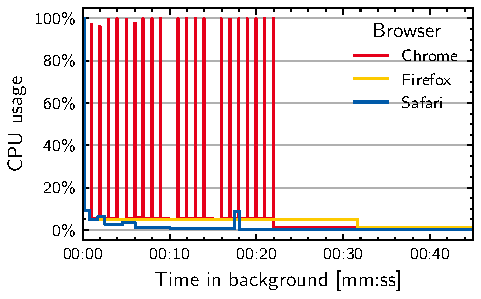
\includegraphics[width=\textwidth]{images/timer-50.pdf}
      \caption{50 ms task duration}
    \end{subfigure}
    \hfill
    \begin{subfigure}[t]{0.5\textwidth}
      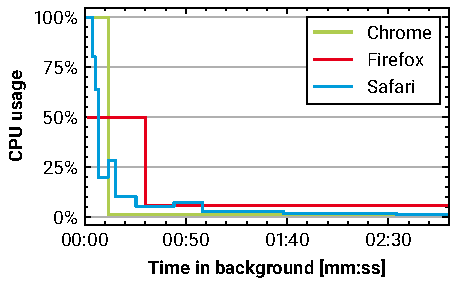
\includegraphics[width=\textwidth]{images/timer-1000.pdf}
      \caption{1000 ms task duration}
    \end{subfigure}

    \caption{CPU usage over time for continuously scheduled timer tasks in background tabs}
    \label{fig:timer}
  \end{figure}

  \subsection{Timer tasks with WebSocket / AudioContext}

  Browser vendors try to strike a balance between throttling background pages as much as possible to conserve energy and keep the system more responsive and not breaking existing web applications. As backwards compatibility is an important factor, some browsers reduce their throttling, when they detect, that a web application might need more background processing time. The detection, if a web site needs more processing time is difficult though. Due to the dynamic nature of JavaScript, static analysis of web scripts is very difficult. Therefore browsers use a simple heuristic, to determine if their default throttling should be reduced. Again, we measured and observed the behaviour with our measurement framework. The results of desktop browsers are shown in figure \ref{fig:websocket}.

  Chrome disables the budget-based throttling, when a web site has either an open WebSocket connection open or plays audible music. Playing silent music does not count as audible music playback though \cite{chrome-background-tabs}. This behaviour could be misused to get more processing time for JavaScript tasks. Playing a audbile sound file or opening a WebSocket connection work equalliy in preventing the budget-based throttling, but they differ hugely in how visible they are to the user of the web page. Playing audio is obviously audible and marks your tab with a speaker icon in the tab bar. This is a convenience feature for users to quickly find out, which tab is producing the sounds and is especially useful, if you have many tabs open at the same time. However, Opening a websocket connection is invisible to the user and requires no user confirmation. Additionally Chrome prevents automatic playback of audio unless the user has interacted with the site before or the web site is explicitly whitelisted as a web site with a high media engagement index \cite{chrome-media-engagement-index}. This index is used by Chrome to determine, if a web site can allow audible media autoplay and is generated by the users browsing activity. On a new installation of Chrome, this list is prepopulated with over 1000 sites which Google determined to have a high average media engagement index of all Chrome users \cite{chrome-autoplay}. Chrome on Android behaves exactly the same as Chrome for desktop except for the 5 minute limit as described in section \ref{sec:timer-tasks}.

  Firefox also disables the budget-based throttling when a open WebSocket connection is active, but the limitation of 1 task invocation per second stays intact. However, Firefox does completely disable all timer throttling when an AudioContext was opened on the web site since Firefox version 51 \cite{firefox-audiocontext-exemption}. We could observe and replicate this behaviour on Firefox for desktop as well as Firefox for Android, even when no audible audio was playing at all. Opening an AudioContext does not require special user permission and allowed us to saturate the main thread with an average CPU usage close to 100 \%. With this method, we can completely bypass all energy conserving methods on Firefox.

  Safaris behaviour does not change, when a WebSocket connection is active or an AudioContext was opened, neither for Safari for Mac nor for Mobile Safari for iOS.

  \begin{figure}
    \begin{subfigure}[t]{0.5\textwidth}
      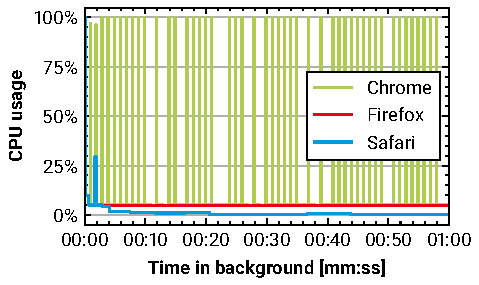
\includegraphics[width=\textwidth]{images/websocket-50.pdf}
      \caption{50 ms task duration}
    \end{subfigure}
    \hfill
    \begin{subfigure}[t]{0.5\textwidth}
      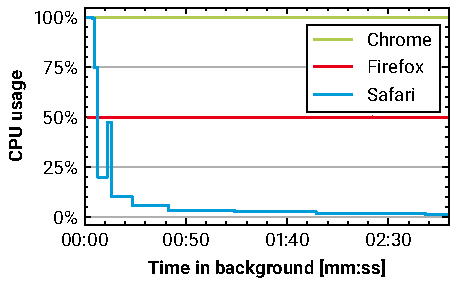
\includegraphics[width=\textwidth]{images/websocket-1000.pdf}
      \caption{1000 ms task duration}
    \end{subfigure}

    \caption{CPU usage over time for continuously scheduled timer tasks in background tabs with an open WebSocket connection}
    \label{fig:websocket}
  \end{figure}



  \subsection{\texttt{postMessage()} tasks}

  Besides \texttt{setTimeout()} or \texttt{setInterval()} there exists another API for putting tasks in the JavaScript task queue. The function \texttt{postMessage()} available on the window and worker scope is available to allow for communication between windows of different origins or between main thread and worker thread \cite{mdn-postmessage}. As each window or worker has its own JavaScript execution context, the communication between these context must happen explicitly via \texttt{postMessage()} calls. The receiving context has to register for the \texttt{message} event on the window or worker object. A call to \texttt{postMessage()} with the receiver set to a window or worker who registered for the event, adds a new task to the task queue for this window. The scheduling of tasks, which are created with the before mentioned method, are not subject to the throttling as explained in the timer tasks section. This is also true for when a \texttt{postmessage()} call is sent and received from the same context. Tasks created with this method are also not subject to the minimum delay of 4 ms as timer tasks are \cite{zero-delay-timeouts}.

  All desktop browsers do not throttle the scheduling of task created via \texttt{postMessage()}. This allows a web site to fully utilize the CPU even when it is on the background. Chrome and Firefox allow to use this method to run indefinitely, whereas Safari detects that a web page is using significant energy and reloads the page after around 8 minutes in the background.

  
  \subsection{Web workers}

  Web workers allow us to spawn a seperate execution context, which behaves different then the main execution context \cite{mdn-worker}. Worker contexts are also treated differently by browsers with regards to timer throttling in the background. Timers created with \texttt{setInterval()} or \texttt{setTimeout()} inside the worker context are not subject to the throttling when the corresponding web page moves to the background. This fact is used by the library worker-timers \cite{worker-timers}, which implements a broker and scheduler for timer tasks which are not throttled when the page moves to the background. The scheduler component runs inside the web worker, whereas the broker is run from the main execution context and dispatches messages when a timer was created or cleared via \texttt{postMessage()} to the worker context. The scheduler then sets an appropriate interval inside the worker context. When the timer inside the worker context fires, the scheduler posts a message to the main thread, which then calls the scheduled function. Through this indirection, the main thread can schedule timers with the worker-timers library, as if it was using the native window timers, but without the throttling behaviour, when the page is in the background. We created a test case with our measuring framework, how each browser behaves with this workaround.
  
  Chrome and Firefox do not throttle timers in web worker context for background tabs at all. This means you can max out the main thread context with the worker-timers library for indefinite time.

  Safari does also not throttle timers in web worker context for background tabs, but it will detect significant energy usage and may reload the page after constant time with high CPU usage. There is also a feature in the macOS operating system called AppNap, which might suspend the browser at whole, when Safari itself is not visible to the user \cite{osx-app-nap}. This feature kicks in, when the operating system decides, that the browser does not provide critical functionality at the moment and is also not visible. When the user is interacting with the Safari, but not the background tab itself then AppNap will not be invoked.
  

  \section{Extensibility}

  We have limited our detailed analysis of background execution methods to these methods listed above, but the measuring framework we developed can be used for further investigation of other methods to achieve arbitrary background execution.

  \subsection{Future browser updates and new APIs}

  Chrome and Firefox have adopted a rapid release cycle with new major releases of their product every couple weeks. When new versions are released with new energy conserving features, our research can be reliablty be verified with these new browser versions. Additionally with every major update, browser may ship new experimental APIs, which can be investigated for achieving background execution. These experimental and browser specific APIs may become a new HTML5 standard API. This is also a trend which emerged in the last years. New HTML5 standardization usually emerges by a browser implementing new features in a vendor specific API. When this API is proven to be useful and accepted by web site authors, it is converted to a API design specification to be implemented by other browsers.
  
  \subsection{Service workers}

  A notable omission to our detailed analysis are service workers. Although they have a similar name as web workers, they serve a complete different purpose. Service workers are complementary scripts, which belong to an URL for which they are registered. The service worker is invoked by the browser in response to certain events, which can be triggered by the website but also by the browser or the server which hosts the web site. Service workers are decoupled from the lifetime of the web page which registered the service worker. If two tabs of the same page are open, only one service worker is used by the browser to handle the events for these two tabs. The main use cases for service workers at the moment are a) providing a offline capable web site and b) allowing web site push notifications. To implement offline capable web sites, the service worker registers for intercepting network requests from the web site. If the user is offline and tries to do a network request, the service worker uses a cached response to handle the request or saves the payload for sending it later, when the user is online again. Service workers try to close the gap between web and native applications and may be extended to support more functionality.

  We omitted the analysis of service workers, because the service workers specifications explicitly recommends, to terminate service workers which take longer then expected to perform their respective tasks. It could be possible, that browser implementations to not adhere to this recommendation, but this should be considered a browser bug and not intended behaviour. Our reseach instead focusses on the circumvention of battery conserving features of the browser implementations.


  
  \section{Summary}

  In this section we analysed the behaviour of background tabs for desktop and mobile browsers. We saw that all browsers employ a timer throttling when the page is in the background. Chrome and Firefox use a budget-based timer throttling approach, whereas Safari increases the time between timer calls with every invocation. The timer throttling of all browsers can be circumvented by using the \texttt{postMessage()} API or by using web workers. Additionally, Chrome's throttling can be disabled by opening a websocket connection and the throttling in Firefox can be disabled by opening an AudioContext. With all circumvention methods, we can saturate the main thread for indefinite amount of time in Chrome and Firefox. Only Safari detects continuous high CPU usage and reloads the page when it is using significant energy. Table \ref{tab:desktop-browser-background} summarizes the findings for desktops browsers.

  These methods could be used by a malicous entity to perform long running background activities. This shows that the throttling mechanisms put in place by browser vendors can only be considered for conserving energy for well-behaving websites and not for protecting the users web sites which actively try to circumvent the throttling.

  The behaviour of mobile browsers differ in some aspects to their desktop counterparts. Mobile Safari completely suspends background tabs as soon as the user switches to another tab. Chrome for Android limits the scheduling of tasks to a maximum of five minutes when the page is in the background. We could not detect a change of behaviour of Firefox for Android to the desktop version of Firefox.

  \begin{table}
    \centering
    \begin{adjustbox}{angle=90}

      \begin{tabularx}{\textheight}{ p{3cm} | X | X | X }
        \toprule
       \thead{Method}              & \thead{Chrome} & \thead{Firefox} & \thead{Safari}                   \\
      \midrule
      Timer tasks                  & Coalesced invocations at most once per second. Budget-based throttling after 10 seconds in background.
                                   & Next invocation at least one second after last invocation. Capped budget-based throttling after 30 seconds in background.
                                   & Coalesced invocations. Time between invocations increases.          \\
      \midrule
      Timer tasks with WebSocket
                                   & Coalesced invocations at most once per second. No budget-based throttling.
                                   & Next invocation at least one second after last invocation. No budget-based throttling.
                                   & Coalesced invocations. Time between invocations increases.          \\
      \midrule
      Timer task with AudioContext
                                   & Coalesced invocations at most once per second. Budget-based throttling after 10 seconds in background.
                                   & No throttling
                                   & Coalesced invocations. Time between invocations increases.          \\
      \midrule
      \texttt{postMessage()} tasks & No throttling
                                   & No throttling
                                   & No throttling, but page gets reloaded when using significant energy \\
      \midrule
      Web worker timer tasks       & No throttling
                                   & No throttling
                                   & No throttling, but page gets reloaded when using significant energy \\
        \bottomrule
    \end{tabularx}
  \end{adjustbox}
  \caption{Summary of desktop browser background tab behaviour}
  \label{tab:desktop-browser-background}
\end{table}

 

  \newpage
  \chapter{Tracing of background execution on popular websites}
  \label{chap:tracing}

  In the first part of our research we identified different methods to circumvent the browser timer throttling mechanisms for brackground tabs. With these findings in mind we can now trace popular websites to analyse if these circumenvtion methods are used in the wild. We used the first 1500 web sites included in the last free publication of the Alexa top 1 million site list\footnote{The list is available under \url{http://s3.amazonaws.com/alexa-static/top-1m.csv.zip}}. We decided to just trace the home page of each web site and no sub pages to limit the scope of this research. This is a known compromise of this tracing research, because many web applications only show a largly static landing page on the home page, while the script-heavy application itself is only available after login. On the other hand, it is not feasable to provide login credentials for a mass analysis of web sites, but it could be the topic of further research in this area. After we visit the home page of the web sites we measure the CPU usage caused by scripting after it was moved to a background tab. With the aggregated result of our tracing, we can determine if the browser throttling mechanisms are suiteable to limit CPU usage or if large number of websites use these methods to actively or inadvertently bypass the background throttling mechanisms of the browser. For this part of our research we focus only on desktop browsers, because the potential for misuse of desktop browsers is much larger. As the browser usage on mobile is limited to smaller timespans, usage of browsers on non-mobile devices is more ubiquitous as more and more applications are replaced with web apps. Often times the browser is open as long as the system itself, with many tabs open in the background during the whole time. The most used desktop browser in the year 2019 is Google Chrome with over 70 \% of market share according to \cite{statcounter-desktop-browser-market-share}. With this leading margin over other browsers, we decided to only trace web sites with Chrome.
  
  \section{Automated measuring of background execution}

  To trace a web site in the background we perform the following steps: First we open a new Chrome instance and start the browsers internal web profiling. Then we open the website to trace and wait for the initial load to complete. After that we move this website to the background by opening a new tab, so that the browser throttling mechanisms are activated. We profile the page for a 15 minutes time period. After the 15 minutes are completed, we close the browser instance and save the website trace for analysis.
    
  To automate the tracing we used Puppeteer \cite{pptr}. Puppeteer is a NodeJS library which uses the Chrome DevTools Protocol \cite{chrome-devtools-protocol} to control a Chrome. The DevTools Protocol is also used by Chrome DevTools which are bundled with Chrome and it allows to access the browser interals. With Puppeteer we can therefore use the same tracing capabilities of Chrome as the web profiler included in the Chrome DevTools. This allows us to evaluate our traces with the existing profiling tools of Chrome. The website trace includes information if the website is executing code and the duration of each JavaScript task that was executed while the web site was in the background.

  Another capability of puppeteer is to inject custom JavaScript code before a web site is rendered. Due to the dynamic nature of JavaScript, it is possible to override the implementation of every existing function. We use this feature in our injected script to hook the API for creating Web workers, opening a WebSocket and using \texttt{postMessage()} calls, to record their respective usage for our tracing. A simplified example how the hooking is performed looks like this:

\begin{lstlisting}
const orig_postMessage = window.postMessage;
window.postMessage = function () {
  console.log('postMessage() was called');
  return orig_postMessage(...arguments);
}
\end{lstlisting}

  To hook a function, we first save the orginal function in a new variable in line 1. We then redefine the function to record the usage in line 3 and pass the arguments the original function in line 4. The \texttt{arguments} object is available in all non-arrow function and refers to the parameters passed to the function. With this hooking technique we can record the calls for APIs, which we are interested in, without the need to change the code of the web sites we trace.

  \section{Analysis of web site traces}
  \label{sec:trace-analysis}

  The trace file generated with Puppeteer consists of a list of events, a corresponding timestamp and the thread and process on which the event took place. With these information, we can reconstruct the timeline of tasks and the stack traces during the recording. To display the timeline, we can use the web profiler embedded in the Chrome DevTools. When we combine this information together with the recoding of the hooked functions during the recording, we can determine which tasks the web site was executing while it was in the background and which methods it used for scheduling the tasks.

  To get a better picture of how web sites in general behave in the background, we need to find a way to compare and aggregate the results of the all traces. To compare the result of two traces, it is beneficial to have a single score for each web site. We propose to use the average CPU usage triggered by scripting during the profiling to use as this score. The average CPU usage score can be calculated from the trace file generated by the web profiler. To calculate the CPU usage time for scripting we use the sum of the duration of all JavaScript tasks executed in the main thread as well as in all potentially spawned worker threads. We use the wall clock time for this measurement, because it is a suitable replacement for CPU time in a scenario where the machine on which the measurements are taken is not under any other load from other processes. Additionally this is the same method which Chrome uses for the budget-based throttling calculation \cite{chrome-background-tabs}. By dividing the summed duration of all tasks with the duration of our trace recording we get the average CPU usage score. A website which uses no JavaScript at all should therefore receive a score of 0, whereas a website which does run uninterupted calculations on the main thread should receive a score of 1. If a website uses multiple worker threads and the machine on which the measurements are taken has more then one physical CPU core, then the website could receive a score which is greater then 1, because all workers could be active at the same time. We also compute the average CPU usage score only considering web worker threads as well as the score for the main thread when a WebSocket connection was open. With these additional scores, we can see if the average shifts, when a circumvention method was used.

  The background throttling mechanism put in place by Google Chrome does limit the timers of websites based on a CPU time budget. This budget is currently set to regenerate at a rate of 0.01 seconds per second \cite{chrome-background-tabs}. That means that websites on average can only use 1 \% of CPU time for scripting. That would also equal a score of 1 \% in our proposed average CPU usage score. This limit gives a good estimation if websites try to overcome the background throttling mechanism of Chrome. Websites which score far greater then 1 \% presumably use one or more methods to prevent the throttling. However, this limit of 1 \% applies per execution context. If a web site includes multiple cross origin iframes, that is frames from a different domain name, than this iframe has its own execution context and therefore its own timer budget. The inclusion of cross origin frames is not quite common in popular web sites, because that is the preferred method of displaying ads. If a web site includes multiple such cross origin iframes, the combined average CPU usage can then far exceed the 1 \% limit put in place by the timer budget.

  
  \section{Evaluation of tracing results}

  \begin{table}
    \begin{adjustbox}{center}
      \begin{tabular}{l r c c r}
        \toprule
        \thead{Web site}   & \thead{Avg. CPU usage} & \thead{WebSocket} & \thead{Worker} & \thead{\texttt{postMessage()} count} \\
        \midrule
        sports.ru          & 21.817 \%              & \FeatureTrue      & \FeatureFalse  & 187                                  \\
        investing.com      & 10.816 \%              & \FeatureTrue      & \FeatureFalse  & 7                                    \\
        nba.com            & 7.956 \%               & \FeatureFalse     & \FeatureTrue   & 391                                  \\
        binance.com        & 7.184 \%               & \FeatureTrue      & \FeatureFalse  & 0                                    \\
        yenisafak.com      & 6.014 \%               & \FeatureTrue      & \FeatureTrue   & 264                                  \\
        mundodeportivo.com & 5.422 \%               & \FeatureFalse     & \FeatureFalse  & 210                                  \\
        yeniakit.com.tr    & 5.389 \%               & \FeatureTrue      & \FeatureTrue   & 895                                  \\
        independent.co.uk  & 5.336 \%               & \FeatureFalse     & \FeatureTrue   & 127                                  \\
        cinecalidad.to     & 5.314 \%               & \FeatureTrue      & \FeatureTrue   & 0                                    \\
        mobafire.com       & 5.199 \%               & \FeatureFalse     & \FeatureFalse  & 111                                  \\
        \bottomrule
      \end{tabular}
    \end{adjustbox}
    \caption{Top ten web sites with highest average CPU usage}
    \label{tab:top-ten-cpu-usage}
  \end{table}

  \begin{figure}
    \centering
    
    \caption{Distribution of average CPU usage in background}
    \label{fig:distribution-cpu-usage}
  \end{figure}

  With the automated tracing script we measured the background activity from 1558 web sites. The ten web sites with the highest CPU activity in the background are listed in table \ref{tab:top-ten-cpu-usage}.

  The distribution of the background CPU usage is shown in figure \ref{fig:distribution-cpu-usage}. Each bin corresponds to 0.5 \% of average CPU activity. If we only consider web sites using at least one WebSocket connection during the recording, we can clearly see a shift of the average CPU activity in the background. This shows that the throttling of timer tasks is only affecting web sites without WebSocket connections.
  

  We manually analysed a random sample set of web sites with background execution higher then 1 \% by opening the corresponding trace file in the Chrome profiler. We discovered that the vast majority of background execution is attributable to advertisement and tracking scripts. We observed two main activities which are done in the background by these scripts. First, they report the user activity to their tracking server. Second they switch out the ads included in the web site to record multiple ad views during one page view. Both of these activites cause many network requests, which are also impacting the energy usage of the web site.
  
  Some news related web sites reload the complete window after a certain amount of time to show the latest content of the home page when a user leaves the tab open for a long time. This is a low effort solution to always show the current content without the need for a dynamic content replacement scripts and can be easily integrated into existing content management systems. A side effect of reloading the page is that the background timer throttling is reset and the first 10 seconds after the reload are not subject to budget limits. As these news related web site often also include third party ad network scripts, these scripts also have to be executed again. The first seconds after the page was loaded are often times the most CPU intensive period during the whole tracing. We observed during our tracing analysis that web sites which reload themselves after a certain amount of time often exceed the timer budget limits by a large margin.


  \textbf{TODO} histogram, How much \% of web sites are above 1 \% of average CPU usage score.

  Only considiring web sites with workers/websockets, how many are above 1 \%

  histogram

  explain that some tracker networks try to update as fast as they can, even static sites which embed ads.

  postmessage calls are heavily used in sites with high cpu score. they enable communication between iframes of different origins. used for web ad network scripts

  biobiochile case study?
  
  
  
  \newpage
  \chapter{Discussion and conclusion}

  As we have seen in chapter \ref{chap:analysis}, the browser throttling mechanisms do not protect users from malicous web sites, which actively try to use CPU time when they are in the background. They can only be regarded as a energy conserving methods for well-behaving web sites. We also showed in chapter \ref{chap:tracing} that these methods are indeed used by popular web sites.

  To protect users from unwanted CPU usage of background tabs, browsers should suspend tabs completely when they are not visible to the user. This goal is already acknowledged from Chrome developers as stated in \cite{chrome-background-tabs-roadmap}. The reason why this change is not yet implemented can be attributed to the missing alternative APIs for legitimate use of background timers. Suspending all background tabs would break these use cases, in which users expect the page to update in the background. Safari implemented a good interim solution by detecting high energy consumption of background tabs and reloading them, when they reach a certain threshold. This solution allows web site to run computation in the background but only if it does impact battery life too much, but it protects users from unwanted CPU usage and battery drain from web miners or other high CPU workloads.

  We propose two possible solutions for browser vendors to let user-chosen web apps not become suspended when in the background while still suspending all other web sites:

  \begin{figure}
    \centering
    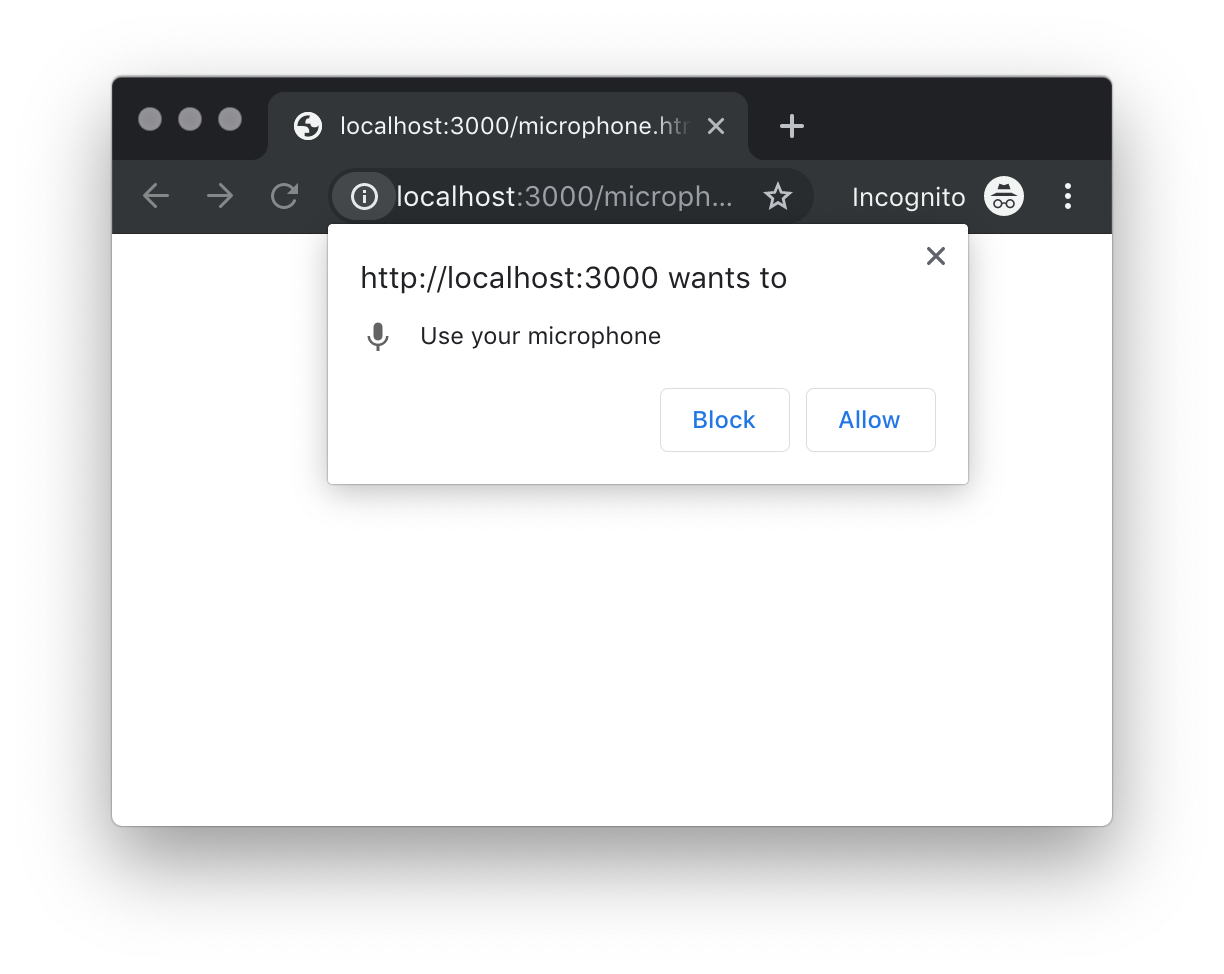
\includegraphics[width=0.5\textwidth]{images/microphone-permission.png}
    \caption{Chrome permission dialog}
    \label{fig:chrome-permission-dialog}
  \end{figure}

  The first proposed solution is to make background execution a permission, which web sites have to explicitly ask for. Browser could then display a popup where users can allow or deny the use of background execution. This popup based permission system is already implemented for other privacy related activities, for example when a web site ask for the users location or access to camera and microphone or when a web site wants to send push notifications. Figure \ref{fig:chrome-permission-dialog} shows how these dialog look like for access to the users microphone. One could argue, that even more permission popups could train users to blindly accept, whatever is shown to them. This behaviour is also reinforced by numerous cookie and policy permission dialogs as implemented to conform to GDPR requirements. On the other hand, cookie and tracking policy permissions are shown inside the web site frame, whereas the proposed background execution permission dialog should be shown from the browser UI and can therefore be recognized as a more important dialog. Web sites would then have to opt in to not be suspended when in the background via a new API. The question remains when this permission popup should be shown two the user. User experience research shows, that users are more likely to deny permission for elevated access, when it is not clear to them, why these permissions are needed \cite{bonne2017exploring}. Therefore, it is considered best practice to not show the permission dialog until the permission is first needed. A good example is the microphone or camera permission dialog. Consider a video conferencing web sites, where these dialogs could be shown, when the users tries to join a call. For background execution permission the natural time, when the web site could ask for this permission is, when the user switches to another tab, but then the context of the web site is already lost and it could be confusing to the user, to then ask for the permission. Another obvious time would be, when the user first visits the web site, but this behaviour contradicts the experience, that users are less likely to give permissions as soon as the web site is loaded. It may not be clear to the user at this time, why the web site needs background execution to function properly. Another approach would be to show the dialog as soon, as the user reopens the tab a couple of times after it was in the background. At that time, it is confirmed, that the user frequently checks the content of this web site. Also the permission dialog could explain to the user, that the content of this page does not refresh in the background without the explicit permission for background execution.

  \begin{figure}
    \centering
    
\includegraphics[width=0.5\textwidth]{images/pinned-tab.png}
    \caption{Pinned tab feature in Safari}
    \label{fig:pinned-tab}
  \end{figure}
  
  The second proposed solution is to disable suspension of tabs, when they are pinned. Pinned tabs is a feature implemented by most desktop browsers, which allows easy access to heavily used web sites. Figure \ref{fig:pinned-tab} displays a pinned tab besides a normal tab in Safari. Pinned tabs usually only show the favicon of the web site and hide the close button of the tab. \cite{firefox-pinned-tabs} explains how pinned tabs work in Firefox. It also describes, why users should use pinned tabs: ``The internet is now full of websites that we use more like programs than just static pages. Popular sites like Facebook and Gmail are like this – they're used to accomplish tasks (or to avoid accomplishing tasks), they update themselves and notify you when they've changed.'' Web sites, which users are likely to pin, are often times the same pages benefiting from background execution. It therefore makes sense, to combine the permission for background execution to pinned tabs. We claim, that the coupling of the background execution permission and pinned tabs is exactly what users expect for pinned tabs. With this solution, users do not have to be asked for another permission and it allows legitimate web sites to perform background tasks while still letting the user be in control of background CPU usage. It would also not require a new API for requesting the background execution permission and is therefore backwards compatible with existing web sites. Pinning a web site tab thereby converts the browser behaviour from a normal web site to a web application.

  Mobile browsers do not have a concept of pinned tabs, but Android and iOS support adding web sites to the home screen. When added to the home screen, a web app can hide the browser chrome for navigation and the address bar to behave more like a fully native app. We propose to give background execution permission to these web sites, which were added to the home screen by the user. This would be the equivalent of a pinned tab on desktop browsers for background execution behaviour.
  

  
  \newpage
  \printbibliography[heading=bibnumbered]


  \affidavit


\end{document}
%%% Local Variables: 
%%% mode: latex 
%%% TeX-engine: luatex
%%% TeX-master: t 
%%% End: